\documentclass[a4paper,12pt,english]{article}
%%%%%%%%%%%%%%%%%%%%%%%%%%%%%%%%%%%%%%%%
\usepackage{cite,citesort}
\usepackage{amsmath,amssymb,amstext,amsfonts,euscript}
\usepackage{vmargin}
\usepackage{array}
\usepackage{epsfig}
\usepackage{setspace}
\usepackage[ansinew]{inputenc}
\usepackage[small,nooneline,bf]{caption2}
%%%%%%%%%%%%%%%%%%%%%%%%%%%%%%%%%%%%%%%%
\setlength{\parindent}{1cm}
\setlength{\parskip}{1.5ex}
\setmarginsrb{20mm}{30mm}{20mm}{30mm}{0pt}{0mm}{0pt}{0mm}
%             l     t     r     b
\makeatletter
  \renewcommand{\@cite}[1]{#1}
\makeatother 
%
\newcolumntype{z}{>$l<$}
%\renewcommand{\thesection}{\Alph{section}}
%%%%%%%%%%%%%%%%%%%%%%%%%%%%%%%%%%%%%%%%
%%%%%%%%%%%%%%%%%%%%%%%%%%%%%%%%%%%%%%%%
\begin{document}
\begin{spacing}{2}
\begin{center}
{\bfseries\large Parity non-conservation contribution\\to the NMR shielding constants of chiral molecules:\\}
\vspace{5mm}
{\bfseries\large A 4-component relativistic study}
\end{center}
%%%%%%%%%%%%%%%%%%%%%%%%%%%%%%%%%%%%%%%%
\begin{center}
Radovan Bast$^\star$, Peter Schwerdtfeger$^\dag$, and Trond Saue$^\star$
\end{center}
%%%%%%%%%%%%%%%%%%%%%%%%%%%%%%%%%%%%%%%%
\begin{center}
$^\star$ {\em\footnotesize Laboratoire de Chimie Quantique, Institut de Chimie de Strasbourg,\\LC3-UMR7177 CNRS/ Universit\'e Louis Pasteur, 4 Rue Blaise Pascal, F-67000 Strasbourg, France}

\noindent $^\dag$ {\em\footnotesize Theoretical and Computational Chemistry Research Centre, Bldg. 44,\\Institute of Fundamental Sciences (IFS), Massey University (Albany Campus),\\Private Bag 102904, North Shore MSC, Auckland, New Zealand}
\end{center}
\begin{center}{\bf Manuscript date: \today}\\\end{center}
%%%%%%%%%%%%%%%%%%%%%%%%%%%%%%%%%%%%%%%
A systematic 4-component relativistic study of the parity non-conservation (PNC) contribution to the (isotropic) NMR shielding constants of chiral molecules is presented for the \emph{P}-enantiomers of the series H$_2$X$_2$ (X = $^{17}$O, $^{33}$S, $^{77}$Se, $^{125}$Te, $^{209}$Po). The PNC contributions are obtained within a linear-response approach at the Hartree-Fock level. A careful design of the basis-sets is necessary. The 4-component relativistic results based on the Dirac-Coulomb Hamiltonian are compared to the non-relativistic L\'evy-Leblond results and those obtained by the spin-free modified Dirac Hamiltonian. The calculations confirm the non-relativistic scaling law $Z^3$ of the PNC contribution with respect to nuclear charge $Z$. However, the calculations also show that the {\it overall} scaling is significantly modified by relativistic effects. The scalar relativistic effect scales as $Z^{4.7}$, whereas the spin-orbit effect, of opposite sign, scales better than $Z^6$ and completely dominates the PNC contribution for the heaviest elements. The presented formalism is expected to be valuable for future search for suitable candidates for the experimental determination of PNC effects in NMR spectra.
%%%%%%%%%%%%%%%%%%%%%%%%%%%%%%%%%%%%%%%%
\section{INTRODUCTION}

\noindent Physics is not symmetric under the parity operation. The breakdown of parity symmetry is caused by the so-called parity non-conservation (PNC) of the electroweak interaction mainly between electrons and nucleons. This breakdown of parity symmetry in physics was first postulated by Lee and Yang [\cite{lee1956physrev}] in 1956 and is today well known in nuclear and particle physics. PNC can be observed for instance in the $\beta$-decay under very low temperature in an external magnetic field (as first performed by Wu \emph{et al.} [\cite{wu1957physrev}]) or in the optical rotation in atomic heavy-metal vapors [\cite{macpherson1991physrevlett,meekhof1993physrevlett,edwards1995physrevlett}].

\par The next logical but ambitious step has been to move the attention towards chemical systems. In the realm of molecular physics the inclusion of the electroweak neutral-current interaction leads to a minute energy difference between the two enantiomers of a chiral molecule. The possible connection between this energy difference and the homochirality in biomolecular life is subject to intensive discussion (e.g. Refs. \cite{quack2002angewcheminted,schwerdtfeger:yamagata,schwerdtfeger:salam}). However, an unequivocal experimental determination of this energy difference between two enantiomers has not been achieved so far despite several claims.

\par While the current search for the experimental manifestation of PNC effects in molecules focuses mainly on differences in the infrared and electronic spectra of chiral molecules (see Ref. \cite{berger} for a review and references therein), their influence on NMR parameters like the shielding tensor or spin-spin coupling constants shows an interesting and possibly complementary alternative despite immense technical obstacles [\cite{barra2001chirality}] which shall not be the subject of this article. Barra, Robert, and Wiesenfeld [\cite{barra1986physletta,barra1988europhyslett,barra1996molphys}] were the first to propose a search for PNC effects in the NMR spectra of chiral molecules. They formulated both the theory within the relativistic and the non-relativistic (NR) framework and performed the first calculations using a relativistically parametrized extended H\"uckel method. Since their pioneer work only very recently a few theoretical \emph{ab initio} studies [\cite{berger2003chemphyschem,lazzeretti2003physreva,weijo2000jchemphys}] have been published.

\par A reinvestigation of this problem by an \emph{ab initio} approach has been deemed necessary since the semi-empirical extended H\"uckel method used by Barra, Robert, and Wiesenfeld [\cite{barra1986physletta,barra1988europhyslett}] is known to underestimate PNC energy differences by about an order of magnitude. Independently Laubender and Berger [\cite{berger2003chemphyschem}] and Soncini \emph{et al.} [\cite{lazzeretti2003physreva}] have published the first \emph{ab initio} calculations of PNC contributions to NMR shielding constants - both of them in a non-relativistic formalism without the inclusion of spin-orbit coupling. Laubender and Berger [\cite{berger2003chemphyschem}] have studied the chiral series H$_2$X$_2$ (X = $^{17}$O, $^{33}$S, $^{77}$Se) and 2-fluorooxirane. Soncini \emph{et al.} [\cite{lazzeretti2003physreva}] have reported a NR gauge-invariant formalism by calculating the PNC contributions for H$_2{^{33}}$S$_2$ and \mbox{m-1,2 dithiin}, presenting expressions for both diamagnetic and paramagnetic contributions to the NMR shielding tensor. Recently, Weijo \emph{et al.} [\cite{weijo2000jchemphys}] have reported a study of PNC contributions to NMR shielding constants and indirect spin-spin coupling constants in chiral halomethanes at the level of Hartree-Fock and density-functional theory. They have shown significant effects of correlation on the PNC contributions.

\par The mentioned publications of other groups conclude with negative results in the sense that the calculated PNC contributions are several orders of magnitude below the present resolution in NMR spectroscopy [\cite{barra2001chirality}]. However, they constitute a very important theoretical frame\-work for the search of suitable candidates. The motivation of our work is to pursue the development of this theoretical methodology by extending it to a 4-component relativistic framework which offers a solid theoretical basis for the treatment of heavy-element compounds and which is found to be very successful in the calculations of PNC energy differences in the infrared spectra [\cite{schwerdtfeger2000physrevlett,schwerdtfeger2002physreva,schwerdtfeger2003physrevlett,schwerdtfeger2004jamchemsoc}]. This will make it possible to verify the scaling of the PNC contribution with respect to the nuclear charge for a series of homologous molecules. This $Z$-scaling ($Z$ is the number of protons) is expected to be much smaller for the PNC contribution to the NMR shielding constants ($Z^2$ - $Z^3$) compared to PNC energy differences ($Z^5$ - $Z^6$).

\par Here we present a systematic 4-component relativistic study of the PNC contribution to the (isotropic) NMR shielding constants of chiral molecules for the \emph{P}-enantiomers of the series H$_2$X$_2$ (X = $^{17}$O, $^{33}$S, $^{77}$Se, $^{125}$Te, $^{209}$Po) using a linear-response approach at the Hartree-Fock level. We will give the Hamiltonian employed in this study as well as its non-relativistic limit (NRL) and compare our results with the work of other authors [\cite{berger2003chemphyschem}] and demonstrate where a NR treatment is justified as well as its limitations. At several points we will emphasize various approximations usually introduced in the derivation of the Hamiltonian. The spin-orbit coupling is naturally included in a 4-component relativistic framework - we will assess its effect by deleting the quaternion imaginary parts of matrix representations of the modified Dirac equation and property gradients as described in \mbox{Refs. \cite{saue2000jchemphys} and \cite{saue2005advquantumchem}}, respectively.

\par The chosen set of molecules is \emph{not} suitable for the experimental search of PNC effects due to stereomutation as already pointed out in Ref. \cite{berger2003chemphyschem}. However, this model set is very well studied from the theoretical point of view and is ideal for a systematic calibration of our implementation which we expect to be valuable for future search of suitable candidates for the experimental determination of PNC effects in NMR spectra.
%%%%%%%%%%%%%%%%%%%%%%%%%%%%%%%%%%%%%%%%
\section{FORMALISM}

\noindent The Hamiltonian employed in this study (\ref{eq:hamiltonian}) for the electroweak neutral-current interaction between electrons and nuclei can be derived from the V-A (vector electron minus axial vector nucleus) Fermi coupling neglecting the momentum transfer between the electrons and the nuclei and consists of nuclear spin-independent ($\hat{h}_\text{pnc}(i)$) and nuclear spin-dependent one-electron \mbox{terms ($\hat{h}_{\text{pnc},\mathbf{I}}(i)$) (\ref{eq:hamiltonian})}. SI-based atomic units are used throughout.

\begin{align}
  \hat{H}_\text{pnc} &= \sum_i\{\hat{h}_\text{pnc}(i)+\hat{h}_{\text{pnc},\mathbf{I}}(i)\}\notag\\
                     &= \frac{G_\text{F}}{\sqrt{2}}\sum_{i,A}\biggl\{\frac{1}{2}Q_\text{w}(A)\gamma^5\rho_A(\mathbf{r}_i)-\lambda_A(1-4\sin^2\theta_\text{W})\boldsymbol{\alpha}\cdot\mathbf{I}_A\rho_A(\mathbf{r}_i)\biggr\}\label{eq:hamiltonian}
\end{align}

\noindent Here the indices $i$ and $A$ run over all electrons and nuclei respectively, $G_\text{F} = 2.22254\cdot 10^{-14}E_ha_0^3$ is the Fermi coupling constant, \mbox{$Q_\text{w}(A) = Z_A(1-4\sin^2\theta_\text{W})-N_A$} is the weak nuclear charge with $Z_A$ and $N_A$ representing the number of protons and neutrons in nucleus $A$, respectively, and $\sin^2\theta_\text{W} = 0.2319$ being the employed Weinberg parameter (the most recent value is $\sin^2\theta_\text{W} = 0.2397(13)$ [\cite{anthony2005physrevlett}]). $\gamma^5$ is one of the Dirac matrices (\ref{eq:gamma5}) with $1_{2\times 2}$ being the $2\times 2$ identity matrix.

\begin{equation}\label{eq:gamma5}
  \gamma^5 = \begin{pmatrix}0_{2\times 2}&1_{2\times 2}\\1_{2\times 2}&0_{2\times 2}\end{pmatrix} \qquad \boldsymbol{\alpha} = \begin{pmatrix}0_{2\times 2}&\boldsymbol{\sigma}\\\boldsymbol{\sigma}&0_{2\times 2}\end{pmatrix}
\end{equation}

\noindent $\rho_A$ is the normalized nuclear charge density, and $\lambda_A$ a nucleus-dependent parameter close to unity [\cite{cahn1977physlettb,marciano1978physrevd,berger}]. $\boldsymbol{\alpha}$ is given in Eq. \ref{eq:gamma5} with $\boldsymbol{\sigma}$ being the Pauli spin matrices in the standard representation. Finally, $\mathbf{I}_A$ is the spin of nucleus $A$. This is only an approximation to the (unknown) nuclear spin density distribution. In the case of a positive experimental measurement the theoretical PNC contribution could be used to reveal or to verify various nuclear spin or charge density distribution models (see e.g [\cite{mukhamedjanov:solidpnc} and references therein).

\par In this paper we will consider only the nuclear spin-dependent part as only the spin-dependent terms $\hat{h}_{\text{pnc},\mathbf{I}}(i)$ will contribute directly to the NMR shielding tensor and therefore we set $\hat{H}_\text{pnc} \equiv \hat{H}_{\text{pnc},\mathbf{I}}$ and obtain our final expression (\ref{eq:hamiltonianPNC}) by replacing the nuclear spin by the nuclear magnetic moment $\mathbf{M}_A = \gamma_A\mathbf{I}_A$, where $\gamma_A$ is the magnetogyric ratio of nucleus $A$.

\begin{equation}\label{eq:hamiltonianPNC}
  \hat{H}_\text{pnc} \equiv \hat{H}_{\text{pnc},\mathbf{I}} = -\frac{G_\text{F}(1-4\sin^2\theta_\text{W})}{\sqrt{2}}\sum_{i,A}\{\frac{1}{\gamma_A}\boldsymbol{\alpha}\cdot\mathbf{M}_A\rho_A(\mathbf{r}_i)\}
\end{equation}

\noindent For comparison with the work of Laubender and Berger [\cite{berger2003chemphyschem}] we have set the nucleus-dependent parameter $\lambda_A \equiv 1.0$. The contribution of the nuclear anapole moment [\cite{zeldovic1958sovphys}] to the PNC shieldings has been neglected as well.

\par For later discussion it will be instructive to consider the NRL of Eq. \ref{eq:hamiltonianPNC}. We employ the NRL of the small component bispinor (\ref{eq:nrl1})
\begin{equation}\label{eq:nrl1}
  \lim_{c\rightarrow\infty}c\vert\psi^\text{S}\rangle = \frac{1}{2m}(\boldsymbol{\sigma}\cdot\mathbf{p})\vert\psi^\text{L}\rangle
\end{equation}
in conjunction with the Dirac identity (\ref{eq:diracidentity}) 
\begin{equation}\label{eq:diracidentity}
  (\boldsymbol{\sigma}\cdot\mathbf{P})(\boldsymbol{\sigma}\cdot\mathbf{Q}) = \mathbf{P}\cdot\mathbf{Q}+\text{i}\boldsymbol{\sigma}\cdot(\mathbf{P}\times\mathbf{Q})
\end{equation}
for arbitrary vectors $\mathbf{P}$ and $\mathbf{Q}$ to obtain
\begin{align}
 \langle\psi\vert(\boldsymbol{\alpha}\cdot\mathbf{M}_A\rho_A(\mathbf{r}_i))\vert\psi\rangle &= \langle\psi^\text{L}\vert(\boldsymbol{\sigma}\cdot\mathbf{M}_A\rho_A(\mathbf{r}_i))\vert\psi^\text{S}\rangle+\langle\psi^\text{S}\vert(\boldsymbol{\sigma}\cdot\mathbf{M}_A\rho_A(\mathbf{r}_i))\vert\psi^\text{L}\rangle\\
  &= \frac{1}{2mc}\bigl\{\langle\psi^\text{L}\vert(\boldsymbol{\sigma}\cdot\mathbf{M}_A\rho_A(\mathbf{r}_i))(\boldsymbol{\sigma}\cdot\mathbf{p})\vert\psi^\text{L}\rangle+\langle\psi^\text{L}\vert(\boldsymbol{\sigma}\cdot\mathbf{p})(\boldsymbol{\sigma}\cdot\mathbf{M}_A\rho_A(\mathbf{r}_i))\vert\psi^\text{L}\rangle\bigr\}.\notag
\end{align}
The NRL can then expressed as
\begin{equation}
  \lim_{c\rightarrow\infty}c\hat{H}_\text{pnc} = -\frac{G_\text{F}(1-4\sin^2\theta_\text{W})}{2\sqrt{2}m}\sum_{i,A}\frac{1}{\gamma_A}\bigl\{\mathbf{M}_A\cdot[\mathbf{p}_i,\delta^3(\mathbf{r}_{iA})]_+-2\text{i}(\mathbf{s}_i\times\mathbf{M}_A)\cdot[\mathbf{p}_i,\delta^3(\mathbf{r}_{iA})]\bigr\}.\label{eq:nrl2}
\end{equation}

\noindent Here we have also made the transition from a finite nucleus density $\rho_A(\mathbf{r}_i)$ to a point nucleus contact interaction described by the Dirac distribution $\delta^3(\mathbf{r}_{iA})$ with $\mathbf{r}_{iA} = \mathbf{r}_i-\mathbf{r}_A$. $\mathbf{s} = \boldsymbol{\sigma}/2$ denotes the electron spin, $c$ the speed of light, $[\cdot,\cdot]$ the commutator and $[\cdot,\cdot]_+$ the anticommutator. We have investigated the importance of the usually omitted electron spin-dependent term (second term in Eq. \ref{eq:nrl2}), however zero PNC contribution has been observed.

\par The nuclear magnetic shielding is defined as the second derivative of the energy with respect to the nuclear magnetic moment $\mathbf{M}_A$ and the external uniform magnetic field $\mathbf{B}$ at zero perturbation strength:

\begin{equation}\label{eq:shielding}
  \sigma_{A,\epsilon\tau} = \frac{\partial^2E(\mathbf{M}_A,\mathbf{B})}{\partial{M_{A,\epsilon}}\partial{B_\tau}}\biggr|_{\mathbf{M}_A=\mathbf{0},\;\mathbf{B}=\mathbf{0}}
\end{equation}

\noindent At the 4-component relativistic level the operator associated with an external magnetic field is usually chosen as
\begin{equation}
\label{eq:hamiltonianB}
\hat{h}_B=-\frac{c}{2}\mathbf{B}\cdot\sum_i\left(\boldsymbol{\alpha}\times\mathbf{r}_{iG}\right)
\quad\text{with} \quad \mathbf{r}_{iG} = \mathbf{r}_i-\mathbf{r}_G,
\end{equation}
where $\mathbf{r}_G$ is the gauge origin. The PNC contribution to the NMR shielding tensor is thereby given by the linear response function
\begin{equation}\label{eq:pncshielding}
  \sigma_{A,\epsilon\tau}^\text{pnc} = -\frac{G_\text{F}(1-4\sin^2\theta_\text{W})}{2\gamma_A\sqrt{2}c_0}\langle\langle c\boldsymbol{\alpha}_\epsilon\rho_A(\mathbf{r}_i));c(\boldsymbol{\alpha}\times\mathbf{r}_{iG})_\tau\rangle\rangle_{\omega=0} 
\end{equation}

\noindent In Eq. \ref{eq:pncshielding} two different $c$ appear ($c$ and $c_0$). By varying $c \rightarrow \infty$ the fixed $c_0 = 137.036$ a.u. guarantees the NRL employed in the literature. We will make use of this technique later in this article. Note, however, that in the strict NRL the PNC contribution (as well as the shielding itself) is zero, as discussed in Ref. \cite{saue2005advquantumchem}.

\par The static linear response function $\langle\langle\hat{H}_A;\hat{H}_B\rangle\rangle_{\omega=0}$ is constructed from property gradients $\mathbf{E}_A^{[1]}$ and $\mathbf{E}_B^{[1]}$ according to

\begin{equation}
  \langle\langle\hat{H}_A;\hat{H}_B\rangle\rangle_{\omega=0} = -\mathbf{E}_A^{[1]\dag}\bigl(E_0^{[2]}\bigr)^{-1}\mathbf{E}_B^{[1]},
\end{equation}

\noindent where $E_0^{[2]}$ is the electronic Hessian . In practice the explicit evaluation of $E_0^{[2]}$ is computationally too demanding and the linear response function is constructed by first solving the response equation
\begin{equation}\label{eq:solution}
  E_0^{[2]}\mathbf{X}_B(\omega) = -\mathbf{E}_B^{[1]}
\end{equation}
by expanding the solution vector $\mathbf{X}_B$ (\ref{eq:solution}) in trial vectors, followed by contraction of $\mathbf{X}_B$ with the property gradient $\mathbf{E}_A^{[1]}$ [\cite{saue:linres}].

\par We will not show in detail how relativistic effects can be eliminated in a 4-component formalism using the spin-free modified Dirac or the L\'evy-Leblond Hamiltonian as this has been done elsewhere [\cite{saue2005advquantumchem}].
%%%%%%%%%%%%%%%%%%%%%%%%%%%%%%%%%%%%%%%%
\section{COMPUTATIONAL DETAILS}

\noindent All calculations have been carried out at the Hartree-Fock level using a development version of the \textsc{dirac} code [\cite{dirac}]. The molecules H$_2$X$_2$ (X = $^{17}$O, $^{33}$S, $^{77}$Se, $^{125}$Te, $^{209}$Po) have been investigated at various dihedral angles with the bond lengths and H-X-X angles kept fixed and taken from Refs. \cite{berger2003chemphyschem} and \cite{peter1999physreva} for comparison. The X$_2$ unit was aligned along the $y$-axis with the dihedral angle bisected by the $yz$-plane. We have used both (contracted) \mbox{aug-cc-pV\{D,T,Q\}Z} basis-sets for H, O, S, and Se as well as the even-tempered basis-sets for O, S, Se, Te, and Po developed by Laerdahl and Schwerdtfeger [\cite{peter1999physreva}] together with uncontracted aug-cc-pVDZ for H. The even-tempered parent set consists of 26 exponents. We will denote these basis-sets as ,,$s$.$p$.$d$.$f$\/'' where $s$, $p$, $d$, and $f$ represent the subsets with the respective angular momenta.

\par The gauge origin has been placed at the center of the nucleus under study (O, S, Se, Te, Po). A Gaussian charge distribution has been chosen as the nuclear model for the Dirac-Coulomb and the spin-free calculations [\cite{luuk:gnuc}]. For comparison with the NR calculations by Laubender and Berger [\cite{berger2003chemphyschem}] point-charge nuclei have been used for the L\'evy-Leblond calculations unless otherwise indicated. The small component basis-set for the calculations based on the Dirac-Coulomb Hamiltonian has been generated using separately unrestricted (UKB) and restricted kinetic balance (RKB) respectively for comparison with the spin-free results. In the Dirac-Coulomb and the spin-free calculations the (SS$\vert$SS) integrals have been eliminated in both the SCF and the linear response part. Their contribution to energies has been modeled by classical Coulombic repulsion of small component atomic charges [\cite{visscher1997theorchemacc}]. 
The response equations (\ref{eq:solution}) have been solved with respect to the property gradient associated 
with the external magnetic field $\mathbf{B}$. Rotations between positive and negative energy solutions 
have been suppressed within the linear response module. This approximation implies neglecting the 
diamagnetic contribution as discussed in Ref. \cite{aucar1999jchemphys}. In the non-relativistic limit
the diamagnetic contribution to the PNC shielding constant is zero, as shown by Soncini \emph{et al.} 
[\cite{lazzeretti2003physreva}]. We find that the inclusion of these rotations alters for instance 
the PNC contribution to the NMR shielding  constant of $^{77}$Se only by 1.3\% (at the dihedral angle of 
45 \textsuperscript{o}). A tight convergence of the response vector is however very important. 
We have used the value $1.0\times 10^{-9}$ as threshold for the ratio of norms between the residual 
and property gradient vectors.
%%%%%%%%%%%%%%%%%%%%%%%%%%%%%%%%%%%%%%%%
\section{RESULTS AND DISCUSSION}

\noindent We have tested our implementation by calculating the PNC contribution to the NMR shielding tensors for the nuclei X = $^{17}$O, $^{33}$S, $^{77}$Se, $^{125}$Te, $^{209}$Po in the \emph{P}-enantiomers of H$_2$X$_2$ for the dihedral angle of 45\textsuperscript{o} at the Hartree-Fock level. These results are reported in Table \ref{ang45}. The PNC contribution is studied using the Dirac-Coulomb (DC) Hamiltonian, the spin-free modified Dirac Hamiltonian, and the L\'evy-Leblond Hamiltonian.

\par The choice of the basis-sets deserves a detailed discussion. In Table \ref{ang45} results for two different classes of basis-sets are reported. We have used aug-cc-pV\{D,T,Q\}Z basis-sets (using their original contraction scheme) in the first instance for comparison with the work of Laubender and Berger [\cite{berger2003chemphyschem}]. We confirm their observation that these basis-sets are not converged without the inclusion of high-exponent \emph{p}-functions (not shown here). For 4-component relativistic calculations of H$_2{^{33}}$S$_2$ and its heavier homologues these basis-sets are qualitatively inappropriate. Rather than correcting these basis-sets by liberating or adding high exponents to the sets we have chosen even-tempered basis-sets with a common parent set as our reference. These even-tempered basis-sets are unbiased and have a greater flexibility in the core \emph{s}- and \emph{p}-region which in practice makes them superior to aug-cc-pVNZ basis-sets for this type of calculation. Somewhat to our surprise we have found that the PNC contribution to the NMR shieldings is not converged with the even-tempered basis sets developed by Laerdahl and Schwerdtfeger [\cite{peter1999physreva}] and that in particular the inclusion of polarizing \emph{f}-functions is important. A representative series of results for H$_2{^{77}}$Se$_2$ obtained during the basis-set optimization for Se is given in Table \ref{Sebas}. The basis-sets for the other elements have been obtained in a similar fashion. They can be considered very close to the basis-set limit within Hartree-Fock. 
\par For the DC calculations two values are given (UKB and RKB) for each combination of molecule and basis-set. The generation of the small component basis-set is usually realized by RKB which is based on the non-relativistic limit of the coupling between the large and small components (\ref{eq:nrl1}). Introducing an external vector potential $\mathbf{A}$ alters however the coupling of large and small components and requires 'magnetic balance' [\cite{aucar1999jchemphys}] such that the use of a small basis-set generated using RKB may lead to substantial errors for NMR shieldings [\cite{saue2004jchemphys}]. This can be corrected by applying UKB, which considers the three components of $\mathbf{p}$ separately and thus provides more flexibility to ensure that the correct coupling can be attained. The difference between UKB and RKB is known to decrease with an increasing quality of the basis-set. We observe identical results for the best performing even-tempered basis-sets for UKB and RKB.

\par For hydrogen going beyond uncontracted aug-cc-pVDZ is not needed. This to some extent indicates the rather atomic nature of this property. Analysis of the linear response functions contributing to the PNC shielding tensor for selenium in H$_2$Se$_2$ shows that they are dominated by orbital rotations between HOMO-LUMO Kramer's partners. Following the projection analysis described in reference [\cite{saue:TlAt}], the relevant molecular orbitals $\psi^\text{mol}_k$ may be decomposed into orbitals $\psi^A_i$ calculated for each constituent atom
\begin{equation}
\vert\psi^\text{mol}_k\rangle = \sum_{i,A}\vert\psi^A_i\rangle c_{ik}^A+\vert\psi^\text{pol}_k\rangle
\end{equation}
where $\psi^\text{pol}_k$ is a polarization contribution which by definition is strictly orthogonal to the 
chosen reference atomic orbitals. Individual gradient elements of a property operator $\hat{\Omega}$ may then be decomposed in intra- and inter-atomic contributions, e.g.
\begin{equation}
\langle\psi_\text{HOMO}\vert\hat{\Omega}\vert\psi_\text{LUMO}\rangle =\sum_{i,A}\sum_{j,B}c_{iA}^{*}c_{jB}\langle\psi_{iA}\vert\hat{\Omega}\vert\psi_{jB}\rangle +(\textrm{polarization})
\end{equation}
We find that the HOMO-LUMO gradient elements of the nuclear spin-dependent PNC operator (\ref{eq:hamiltonianPNC})
are dominated by intra-atomic contributions from the selected selenium center, in particular the Se 4$p_{1/2}$
atomic orbitals coupling with Se 4$s_{1/2}$ and inner Se $s_{1/2}$ AOs. The atomic character of the gradient
elements can be rationalized from the presence of the nuclear charge density $\rho_\text{Se}$ in the operator
which restricts integration to a small volume around the selected selenium center.
Perhaps somewhat less intuitive is the observation that the gradient elements of the property operator
(\ref{eq:hamiltonianB}) associated with the external magnetic field are dominated by intra-atomic contributions
as well, but this is readily understood by the presence of Dirac $\boldsymbol{\alpha}$ matrices in the operator coupling large
and small components. Due to the atomic and very local nature of the small components the gradient elements
are almost exclusively restricted to intra-atomic contributions, but this time from all centers. We find that
the property gradient elements are dominated by intra-atomic coupling  of 4$p_{3/2}$ orbitals on the two
selenium centers. Note, however, that gradient elements coupling occupied positive-energy solutions to 
virtual negative-energy solutions will have a completely different character since the small components
of negative-energy solutions are in fact large and delocalized.

\par Analyzing the values given in Table \ref{ang45} we state that our L\'evy-Leblond results are in excellent agreement with the NR results reported by Laubender and Berger [\cite{berger2003chemphyschem}]. The L\'evy-Leblond PNC contributions are throughout largest in magnitude for the even-tempered basis-sets and larger than the best (modified 5Z) basis-sets used in Ref. \cite{berger2003chemphyschem} (not shown here). For the NR treatment of H$_2{^{77}}$Se$_2$ we have furthermore examined the difference between a point-charge model and a Gaussian model for the nucleus (Table \ref{varang}). The difference is less than 1\%. 
\par Table \ref{varang} shows results for the nuclei X = $^{17}$O, $^{33}$S, $^{77}$Se, $^{125}$Te in H$_2$X$_2$ for various dihedral angles. Only the results for the even-tempered basis-sets are given. The PNC shielding constant is bound to be zero at the dihedral angles 0 $^\circ$ and 180 $^\circ$ due to mirror symmetry. The sinusoidal trait for the dihedral angles between 0 and 180 $^\circ$ is typical and well known also for PNC energy differences or optical rotation. The zero-crossing is usually found near 90 $^\circ$. 


\par A direct comparison of the Dirac-Coulomb (UKB) and the L\'evy-Leblond results in \mbox{Table \ref{ang45}} 
shows that relativistic effects are negligible for H$_2{^{17}}$O$_2$ (-6.064$\times 10^{-9}$ 
ppm R vs. -6.121$\times 10^{-9}$ ppm NR . Also for H$_2{^{33}}$S$_2$ 
the inclusion of relativity is not necessary for qualitative results. The deviation is only 2\% 
(9.977$\times 10^{-8}$ ppm R vs. 9.748$\times 10^{-8}$ ppm NR). For H$_2{^{77}}$Se$_2$ and its heavier homologues on the other hand the discrepancy is evident. For 
these systems an appropriate inclusion of relativistic effects is substantial even for a qualitative 
treatment. For $^{77}$Se, $^{125}$Te, and $^{209}$Po a relativistic treatment even changes the sign 
of the PNC shielding constant at several dihedral angles, as seen in Table \ref{varang}. 
More insight can be gained by looking at 
the individual diagonal components of the PNC shielding tensor, as shown for H$_2{^{77}}$Se$_2$ at
dihedral angle 45\textsuperscript{o} in Table \ref{parcomp}. For all Hamiltonians the $xx$- and $zz$-components
have opposite sign. The smaller $yy$-component changes sign upon inclusion of spin-orbit interaction,
but scalar relativistic effects are non-negligible as well.
\par In figure \ref{cvar} we trace the PNC shielding shielding constant $\sigma^\text{pnc}$ as well 
as $\sigma_{yy}^\text{pnc}$ and $(\sigma_{xx}^\text{pnc}+\sigma_{zz}^\text{pnc})/2$ of $^{77}$Se in 
H$_2$Se$_2$ at dihedral angle 45\textsuperscript{o}, at variable speeds of light and with or without 
the inclusion of spin-orbit coupling. At large values of $c$ the components go smoothly into the 
non-relativistic result. The spin-free results are positive for all values of $c$ and increase significantly
for small values of $c$. However, this effect is completely quenched by a dramatic spin-orbit effect of
opposite sign under ultra-relativistic conditions ($c$ $<$ 137.036 a.u.). We indeed observe for
$^{209}$Po that whereas scalar relativistic effects increase the shielding constant from $9.953\times10^{-7 }$ to
$5.246\times 10^{-6 }$ ppm, spin-orbit coupling amplifies the value by three orders of magnitude to
$-1.277\times 10^{-3 }$ ppm. This corresponds to a line-splitting of about 30 mHz at a magnetic field of 1 Tesla. This means a difference larger than the maximal theoretical resolution of 6 mHz [\cite{barra2001chirality}]. We will in a future publication elucidate these mechanisms by means of
projection analysis.
\par The opposing trends of scalar relativistic and spin-orbit effects make it difficult to extract 
an overall scaling of the PNC shielding constant with respect to nuclear charge $Z$. Table \ref{redpar} shows the 
PNC contributions to the reduced (isotropic) NMR shielding constants 
$\sigma_A^\text{pnc}/\gamma_A$ for the different nuclei. Our values confirm the NR $Z$-scaling law 2-3 
(here: 2.4) observed by Laubender and Berger [\cite{berger2003chemphyschem}], but the non-relativistic
contribution is soon overtaken by the scalar relativistic contribution scaling as $Z^{4.7}$. For the heavier
elements the PNC shielding is however completely dominated by the large and negative 
spin-orbit contribution which scales better than $Z^6$.
% Comparing DC, SF and LL results we identify spin-orbit effects (difference between DC and SF) as dominating for H$_2{^{77}}$Se$_2$, H$_2{^{125}}$Te$_2$, and H$_2{^{209}}$Po$_2$ and opposite to scalar relativistic effects (SR, difference between SF and LL). To illustrate the contributions due to scalar relativistic effects and due to spin-orbit coupling (SO) Table \ref{redpar} shows the PNC contributions to a $\gamma_A$-isolated (isotropic) NMR shielding constants $\gamma_A\sigma_A^\text{pnc} = \gamma_A(\sigma_{A,xx}^\text{pnc}+\sigma_{A,yy}^\text{pnc}+\sigma_{A,zz}^\text{pnc})/3$ for the different nuclei. The opposing effects of scalar relativity and spin-orbit coupling can be clearly seen. In the case of H$_2{^{33}}$S$_2$ these effects almost cancel. This is not true for the heavier homologues where their sum surpasses the NR value and becomes qualitatively significant. Based on these values we confirm the NR $Z$-scaling law 2-3 (here: 2.4) observed by Laubender and Berger [\cite{berger2003chemphyschem}]. This becomes however rapidly quenched by the pronounced scaling due to relativistic effects (4.7 for SR and 6.??? for SO in the opposite direction).


%\par A variation of the speed of light allows to study the PNC contribution under ultra- ($c$ $<$ 137.036 a.u.) or infra-relativistic ($c$ $>$ 137.036 a.u.) conditions (Figure \ref{figure}). The results obtained by this technique go to the correct (LL) NRL, which is reached already at about $c$ = 500 a.u. For values larger than 1000 a.u. numerical instabilities have been observed. Below 100 a.u. strong oscillation is observed. Following this graph a hypothetical situation where the PNC contribution is zero exists for $c$ slightly higher than $c_0$ = 137.036 a.u..
%%%%%%%%%%%%%%%%%%%%%%%%%%%%%%%%%%%%%%%%
\section{CONCLUSION}

\noindent We have studied the importance of relativistic effects on the calculation of the PNC contribution to the (isotropic) NMR shielding constants for the nuclei X = $^{17}$O, $^{33}$S, $^{77}$Se, $^{125}$Te, $^{209}$Po in H$_2$X$_2$ at the Hartree-Fock level. Comparing the results obtained within the Dirac-Coulomb formalism and approximate frameworks with either spin-orbit effects or all relativistic effects eliminated it has been observed that spin-orbit effects are substantial even for a qualitative treatment already for H$_2{^{77}}$Se$_2$ causing a sign change of the PNC contribution. This dramatic difference will be subject of a detailed analysis in a forthcoming paper where also correlation effects will be addressed.

\par We aim to apply the presented methodology for the study of more realistic systems with more rigid structures (as already discussed by Laubender and Berger [\cite{berger2003chemphyschem}]). While the NMR technique seems to impose more experimental boundary conditions than high-resolution infrared spectroscopy experiments [\cite{barra2001chirality}] it offers a possibly complementary approach for the first experimental verification. Our results encourage to include the NMR spectroscopy in the search for the experimental verification and strongly favor heavy-element containing molecules for such NMR experiments. The more promising systems are often considerably larger than the presented set of molecules which might require the use of more efficient (two-component) Hamiltonians.
%%%%%%%%%%%%%%%%%%%%%%%%%%%%%%%%%%%%%%%%
\section{ACKNOWLEDGMENT}

RB gratefully acknowledges financial support by the Conseil R\'egional d'Alsace through the Bourse R\'egionale and by the Fonds der Chemischen Industrie through the Kekul\'e scholarship. TS gratefully acknowledges support from the Royal Society of New Zealand to visit Auckland University. The authors acknowledge valuable discussions with Robert Berger and Pekka Manninen. This work is part of the project {\sc pncmol} funded by the Agence 
Nationale de la Recherche (ANR), France.
\end{spacing}
%%%%%%%%%%%%%%%%%%%%%%%%%%%%%%%%%%%%%%%%
\newpage
%\bibliographystyle{prsty}
\bibliographystyle{aip}
\bibliography{pncnmr}
%%%%%%%%%%%%%%%%%%%%%%%%%%%%%%%%%%%%%%%%
\begin{table}[h]
  \begin{center}
    \caption{
    \label{ang45}
    \emph{
PNC NMR shielding constants (in ppm)
of the nuclei X = $^{17}$O, $^{33}$S, $^{77}$Se, $^{125}$Te, $^{209}$Po
in the P-enantiomers of H$_2$X$_2$
for the dihedral angle of 45 \textsuperscript{o}.
DC denotes the Dirac-Coulomb Hamiltonian,
UKB and RKB the application of unrestricted and restricted kinetic balance respectively,
SF the use of the spin-free modified Dirac Hamiltonian,
LL the use of the L\'evy-Leblond Hamiltonian.
PC denotes a point-charge model for the nucleus.
    }}
    \begin{tabular}{ccr@{\hspace{1pt}}!{$\times$10}@{\hspace{1pt}}zr@{\hspace{1pt}}!{$\times$10}@{\hspace{1pt}}zr@{\hspace{1pt}}!{$\times$10}@{\hspace{1pt}}zr@{\hspace{1pt}}!{$\times$10}@{\hspace{1pt}}z}
      \\
      \hline\hline
      \\
                            &basis-set
                            &\multicolumn{2}{c}{DC(UKB)}
                            &\multicolumn{2}{c}{DC(RKB)}
                            &\multicolumn{2}{c}{SF}
                            &\multicolumn{2}{c}{LL(PC)}\\
      \\
      \hline
      \\
      H$_2{^{17}}$O$_2$
      &aug-cc-pVDZ          & 3.832&^{-9 }& 4.913&^{-9 }& 3.968&^{-9 }& 3.979&^{-9 }\\
      &aug-cc-pVTZ          & 4.458&^{-9 }& 4.466&^{-9 }& 4.616&^{-9 }& 4.600&^{-9 }\\
      &aug-cc-pVQZ          & 4.913&^{-9 }& 4.926&^{-9 }& 5.090&^{-9 }& 5.067&^{-9 }\\
      &1-25.2-26.20-24.20-24& 6.064&^{-9 }& 6.064&^{-9 }& 6.229&^{-9 }& 6.121&^{-9 }\\
      \\
      \hline
      \\
      H$_2{^{33}}$S$_2$
      &aug-cc-pVDZ          &-6.348&^{-8 }&-6.460&^{-8 }&-7.011&^{-8 }&-7.100&^{-8 }\\
      &aug-cc-pVTZ          &-7.187&^{-8 }&-7.351&^{-8 }&-7.948&^{-8 }&-8.036&^{-8 }\\
      &aug-cc-pVQZ          &-7.235&^{-8 }&-7.525&^{-8 }&-8.141&^{-8 }&-8.215&^{-8 }\\
      &1-25.2-26.20-24.20-24&-9.977&^{-8 }&-9.977&^{-8 }&-1.049&^{-7 }&-9.748&^{-8 }\\
      \\
      \hline
      \\
      H$_2{^{77}}$Se$_2$
      &aug-cc-pVDZ          &-2.367&^{-8 }&-2.403&^{-8 }&-1.438&^{-7 }&-1.652&^{-7 }\\
      &aug-cc-pVTZ          &-2.674&^{-8 }&-2.803&^{-8 }&-1.725&^{-7 }&-1.797&^{-7 }\\
      &aug-cc-pVQZ          &-2.172&^{-8 }&-2.573&^{-8 }&-1.883&^{-7 }&-1.866&^{-7 }\\
      &1-25.2-26.15-25.20-24& 1.255&^{-8 }& 1.255&^{-8 }&-2.719&^{-7 }&-2.005&^{-7 }\\
      \\
      \hline
      \\
      H$_2{^{125}}$Te$_2$
      &1-25.2-26.15-25.19-25&-1.295&^{-6 }&-1.295&^{-6 }& 6.128&^{-7 }& 3.146&^{-7 }\\
      \\
      \hline
      \\
      H$_2{^{209}}$Po$_2$
      &1-25.2-26.12-25.15-24& 1.277&^{-3 }& 1.276&^{-3 }&-5.246&^{-6 }&-9.953&^{-7 }\\
      \\
      \hline\hline
    \end{tabular}
  \end{center}
\end{table}

\begin{table}[h]
  \begin{center}
    \caption{
    \label{Sebas}
    \emph{
Basis-set dependence of the Dirac-Coulomb unrestricted kinetic balance
PNC NMR shielding constant (in ppm)
of the nucleus $^{77}$Se
in the P-enantiomer of H$_2$Se$_2$
for the dihedral angle of 45 \textsuperscript{o}.
The basis-set 1-25.2-26.15-25.20-24 has been chosen for further calculations.
    }}
    \begin{tabular}{lr}
      \\
      \hline\hline
      \\
      basis-set\\
      \\
      \hline
      \\
      1-25.2-26.15-25      & 3.156$\times 10^{-8}$\\
      \\
      1-25.2-26.15-25.21-23& 1.224$\times 10^{-8}$\\
      1-25.2-26.15-25.20-24& 1.255$\times 10^{-8}$\\
      1-25.2-26.15-25.19-25& 1.252$\times 10^{-8}$\\
      \\
      1-25.2-26.13-25.21-23& 1.223$\times 10^{-8}$\\
      1-25.2-26.15-26.21-23& 1.221$\times 10^{-8}$\\
      \\
      \hline\hline
    \end{tabular}
  \end{center}
\end{table}

\begin{table}[h]
  \begin{center}
    \caption{
    \label{varang}
    \emph{
PNC NMR shielding constants (in ppm)
of the nuclei X = $^{17}$O, $^{33}$S, $^{77}$Se, $^{125}$Te, $^{209}$Po
in the P-enantiomers of H$_2$X$_2$
for various dihedral angles.
DC denotes the Dirac-Coulomb Hamiltonian,
UKB the application of unrestricted kinetic balance,
LL the use of the L\'evy-Leblond Hamiltonian.
PC denotes a point-charge model,
GM a Gaussian model for the nucleus.
The basis-sets are 1-25.2-26.20-24.20-24 for O,
1-25.2-26.15-25.20-24 for S and Se,
1-25.2-26.15-25.19-25 for Te,
and 1-25.2-26.12-25.15-24 for Po.
    }}
    \begin{tabular}{cr@{\hspace{1pt}}!{$\times$10}@{\hspace{1pt}}zr@{\hspace{1pt}}!{$\times$10}@{\hspace{1pt}}zr@{\hspace{1pt}}!{$\times$10}@{\hspace{1pt}}zr@{\hspace{1pt}}!{$\times$10}@{\hspace{1pt}}zr@{\hspace{1pt}}!{$\times$10}@{\hspace{1pt}}zr@{\hspace{1pt}}!{$\times$10}@{\hspace{1pt}}z}
      \\
      \hline\hline
      \\
      &\multicolumn{2}{c}{30 \textsuperscript{o}}
      &\multicolumn{2}{c}{45 \textsuperscript{o}}
      &\multicolumn{2}{c}{60 \textsuperscript{o}}
      &\multicolumn{2}{c}{90 \textsuperscript{o}}
      &\multicolumn{2}{c}{120 \textsuperscript{o}}
      &\multicolumn{2}{c}{150 \textsuperscript{o}}\\
      \\
      \hline
      \\
      H$_2{^{17}}$O$_2$\\
      \\
      DC(UKB)
             & 5.306&^{-9 }
             & 6.064&^{-9 }
             & 5.219&^{-9 }
             & 1.634&^{-10}
             &-4.812&^{-9 }
             &-4.888&^{-9 }\\
      LL(PC)
             & 5.355&^{-9 }
             & 6.121&^{-9 }
             & 5.272&^{-9 }
             & 1.652&^{-10}
             &-4.912&^{-9 }
             &-5.023&^{-9 }\\
      \\
      \hline
      \\
      H$_2{^{33}}$S$_2$\\
      \\
      DC(UKB)
             &-8.336&^{-8 }
             &-9.977&^{-8 }
             &-9.532&^{-8 }
             &-3.977&^{-8 }
             & 2.477&^{-8 }
             & 3.806&^{-8 }\\
      LL(PC)
             &-8.251&^{-8 }
             &-9.748&^{-8 }
             &-9.170&^{-8 }
             &-3.533&^{-8 }
             & 2.884&^{-8 }
             & 4.158&^{-8 }\\
      \\
      \hline
      \\
      H$_2{^{77}}$Se$_2$\\
      \\
      DC(UKB)
             & 4.690&^{-8 }
             & 1.255&^{-8 }
             &-3.458&^{-8 }
             &-9.935&^{-8 }
             &-1.502&^{-7 }
             &-1.738&^{-7 }\\
      LL(GM)
             &-1.694&^{-7 }
             &-1.993&^{-7 }
             &-1.841&^{-7 }
             &-5.595&^{-8 }
             & 8.602&^{-8 }
             & 1.091&^{-7 }\\
      LL(PC)
             &-1.704&^{-7 }
             &-2.005&^{-7 }
             &-1.852&^{-7 }
             &-5.629&^{-8 }
             & 8.653&^{-8 }
             & 1.098&^{-7 }\\
      \\
      \hline
      \\
      H$_2{^{125}}$Te$_2$\\
      \\
      DC(UKB)
             &-1.420&^{-6 }
             &-1.295&^{-6 }
             &-8.249&^{-7 }
             & 3.879&^{-7 }
             & 1.590&^{-6 }
             & 2.008&^{-6 }\\
      LL(PC)
             & 2.675&^{-7 }
             & 3.146&^{-7 }
             & 2.915&^{-7 }
             & 9.472&^{-8 }
             &-1.250&^{-7 }
             &-1.640&^{-7 }\\
      \\
      \hline
      \\
      H$_2{^{209}}$Po$_2$\\
      \\
      DC(UKB)
             &-7.244&^{-4 }
             & 1.277&^{-3 }
             & 3.043&^{-4 }
             &-3.086&^{-6 }
             &-3.395&^{-4 }
             & 5.709&^{-4 }\\
      LL(PC)
             &-8.694&^{-7 }
             &-9.953&^{-7 }
             &-9.422&^{-7 }
             &-3.130&^{-7 }
             & 3.932&^{-7 }
             & 5.248&^{-7 }\\
      \\
      \\
      \hline\hline
    \end{tabular}
  \end{center}
\end{table}


\begin{table}[h]
  \begin{center}
    \caption{
    \label{parcomp}
    \emph{
Components $\sigma_{ii}^\text{pnc}$ of the
PNC NMR shielding tensor (in ppm)
of the nucleus $^{77}$Se
in the P-enantiomer of H$_2$Se$_2$
for the dihedral angle of 45 \textsuperscript{o}.
DC denotes the Dirac-Coulomb Hamiltonian,
UKB the application of unrestricted kinetic balance,
SF the use of the spin-free modified Dirac Hamiltonian,
LL the use of the L\'evy-Leblond Hamiltonian.
PC denotes a point-charge model for the nucleus.
    }}
    \begin{tabular}{cr@{\hspace{1pt}}!{$\times$10}@{\hspace{1pt}}zr@{\hspace{1pt}}!{$\times$10}@{\hspace{1pt}}zr@{\hspace{1pt}}!{$\times$10}@{\hspace{1pt}}z}
      \\
      \hline\hline
      \\
             &\multicolumn{2}{c}{DC(UKB)}
             &\multicolumn{2}{c}{SF}
             &\multicolumn{2}{c}{LL(PC)}\\
      \\
      \hline
      \\
      $xx$   &-2.094&^{-6 }&-1.830&^{-6 }&-1.310&^{-6 }\\
      $zz$   & 1.908&^{-6 }& 1.220&^{-6 }& 8.766&^{-7 }\\
      $xx+zz$&-1.867&^{-7 }&-6.105&^{-7 }&-4.330&^{-7 }\\
      $yy$   & 2.244&^{-7 }&-2.052&^{-7 }&-1.686&^{-7 }\\
      \\
      \hline\hline
    \end{tabular}
  \end{center}
\end{table}

\begin{table}[h]
  \begin{center}
    \caption{
    \label{redpar}
    \emph{
Reduced PNC NMR shielding constants
$\gamma_A\sigma_A^\text{pnc} = \gamma_A(\sigma_{A,xx}^\text{pnc}+\sigma_{A,yy}^\text{pnc}+\sigma_{A,zz}^\text{pnc})/3$
(in ppm ????????????)
of the nuclei X = $^{17}$O, $^{33}$S, $^{77}$Se, $^{125}$Te, $^{209}$Po
in the P-enantiomers of H$_2$X$_2$
for the dihedral angle of 45 \textsuperscript{o}.
$Z$ is the number of protons,
LL denotes the use of the L\'evy-Leblond Hamiltonian,
SR is the contribution of scalar relativity (SF-LL),
SO the effect of spin-orbit coupling (DC-SF).
    }}
    \begin{tabular}{cr@{\hspace{1pt}}!{$\times$10}@{\hspace{1pt}}zr@{\hspace{1pt}}!{$\times$10}@{\hspace{1pt}}zr@{\hspace{1pt}}!{$\times$10}@{\hspace{1pt}}zr@{\hspace{1pt}}!{$\times$10}@{\hspace{1pt}}z}
      \\
      \hline\hline
      \\
      $Z$&\multicolumn{2}{c}{LL}
         &\multicolumn{2}{c}{SR}
         &\multicolumn{2}{c}{SO}
         &\multicolumn{2}{c}{SR + SO}\\
      \\
      \hline
      \\
      8 &-1.263&^{-12}&-2.228&^{-14}& 3.404&^{-14}& 1.176&^{-14}\\
      16&-1.139&^{-11}&-8.672&^{-13}& 5.996&^{-13}&-2.677&^{-13}\\
      34&-5.842&^{-11}&-2.081&^{-11}& 8.289&^{-11}& 6.208&^{-11}\\
      52&-1.522&^{-10}&-1.443&^{-10}& 9.232&^{-10}& 7.789&^{-10}\\
      84&-4.188&^{-10}&-1.788&^{-09}& 5.395&^{-07}& 5.377&^{-07}\\
      \\
      \hline\hline
    \end{tabular}
  \end{center}
\end{table}

\begin{figure}
  \centering\epsfig{figure=cvalue.eps,width=\linewidth}
    \caption{
    \label{cvar}
    \emph{
Dependence of the
PNC NMR shielding constant (in ppm)
of the nucleus $^{77}$Se
in the P-enantiomer of H$_2$Se$_2$
for the dihedral angle of 45 \textsuperscript{o}
on the speed of light $c$ (in a.u.).
The symbols ($\times, \bigcirc,$ and $\triangle$) represent
the average trace $\sigma^\text{pnc} = (\sigma_{xx}^\text{pnc}+\sigma_{yy}^\text{pnc}+\sigma_{zz}^\text{pnc})/3$,
$\sigma_{yy}^\text{pnc}$,
and $(\sigma_{xx}^\text{pnc}+\sigma_{zz}^\text{pnc})/2$ respectively.
The vertical dashed line represents the true speed of light of $\approx$ 137 a.u.,
the horizontal dashed line shows the non-relativistic limit (-1.993$\times 10^{-7}$ ppm).
    }}
\end{figure}
%%%%%%%%%%%%%%%%%%%%%%%%%%%%%%%%%%%%%%%%
\end{document}
